\documentclass[border=2pt,svgnames,tikz]{standalone}
\usepackage{fontspec}
\setmainfont{Source Serif 4}
\setsansfont{Source Sans 3}
\setmonofont{Source Code Pro}
\usetikzlibrary{arrows.meta, positioning, calc}

\begin{document}
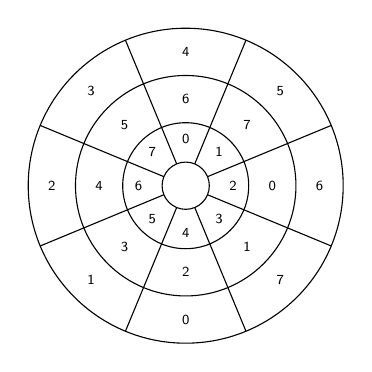
\begin{tikzpicture}[
    sector/.style={draw, fill=white, minimum size=0.5cm, font=\sffamily\tiny},
    track/.style={draw, circle, minimum size=3cm},
    label/.style={font=\sffamily\tiny}
]

% Center point
\coordinate (C) at (0,0);

% Tracks (concentric circles)
\foreach \r in {0.8, 1.4, 2.0} {
    \draw (C) circle (\r);
}

% Sectors
% Inner Track (Track 0)
\foreach \i in {0,...,7} {
    \node[label] at ({90 - \i*45}:0.6) {\i};
    \draw (C) -- ({90 - \i*45 + 22.5}:0.8);
}

% Middle Track (Track 1) - Skewed by 2 sectors
\foreach \i in {0,...,7} {
    \pgfmathsetmacro{\angle}{90 - \i*45 - 2*45}
    \node[label] at (\angle:1.1) {\i};
    \draw ({90 - \i*45 + 22.5}:0.8) -- ({90 - \i*45 + 22.5}:1.4);
}

% Outer Track (Track 2) - Skewed by another 2 sectors (total 4)
\foreach \i in {0,...,7} {
    \pgfmathsetmacro{\angle}{90 - \i*45 - 4*45}
    \node[label] at (\angle:1.7) {\i};
    \draw ({90 - \i*45 + 22.5}:1.4) -- ({90 - \i*45 + 22.5}:2.0);
}

% Spindle
\draw[fill=white] (C) circle (0.3);

\end{tikzpicture}
\end{document}
